\chapter{Threat Model} \label{ch:threat-model}
This chapter contains the threat model established for the system under scrutiny, which was used to identify and document all threats to the system. The methodology and threat model technique is described in section \ref{ch:method:threat-modeling}.

\section{Identified Assets}
As part of the first phase of our threat modeling technique, assets of the system were identified. These can be found in table \ref{tb:assets}.
\begin{table}[!ht]
    \centering
    \begin{tabular}{l}
        \hline
        \textbf{Asset description}
        \\ \hline
        Physical access to the house
        \\
        Personal four-digit pin
        \\
        Arm/disarm state of the system
        \\
        State of triggers, like the sabotage sensors
        \\
        Door contact sensor state
        \\
        Authentication to the admin web application
        \\
        Triggered alarm state
        \\
        Login credentials to the local webserver
        \\ \hline
    \end{tabular}
    \caption{The identified assets of the system.}
    \label{tb:assets}
\end{table}

\section{Architecture Overview}
This section contains an architecture overview of the system. Included in this are three components presented below. First is a list of all identified use cases of the system. The second is a diagram visually presenting all components of the system, how they interact, and the data flow of the system. Lastly, a table of all identified technologies used in the system is presented.

\subsection{Use cases}
As part of the architecture overview, all use cases of the system were identified. These are the use cases a regular user would encounter when using the system normally. The system, from the perspective of a user, is quite simple. The use cases are documented in table \ref{tb:use-cases}.
\begin{table}[!ht]
    \centering
    \begin{tabular}{l}
        \hline
        \textbf{Use case}
        \\ \hline
        The user arms/disarms the system via the remote keypad panel.
        \\
        The user arms/disarms the system via the web portal.
        \\
        The user arms/disarms the system via the mobile app.
        \\
        The user receives a notification about a state change in the system.
        \\
        The user requests a photo be taken by the camera.
        \\ \hline
    \end{tabular}
    \caption{Use cases of the system.}
    \label{tb:use-cases}
\end{table}

\subsection{Architecture diagram}
Figure \ref{fig:system-overview} presents a visual overview of the system, from a technical perspective. All identified components of the system are included, as well as how they all communicate, with what protocol, etc.
\begin{figure}[!p]
    \centering
    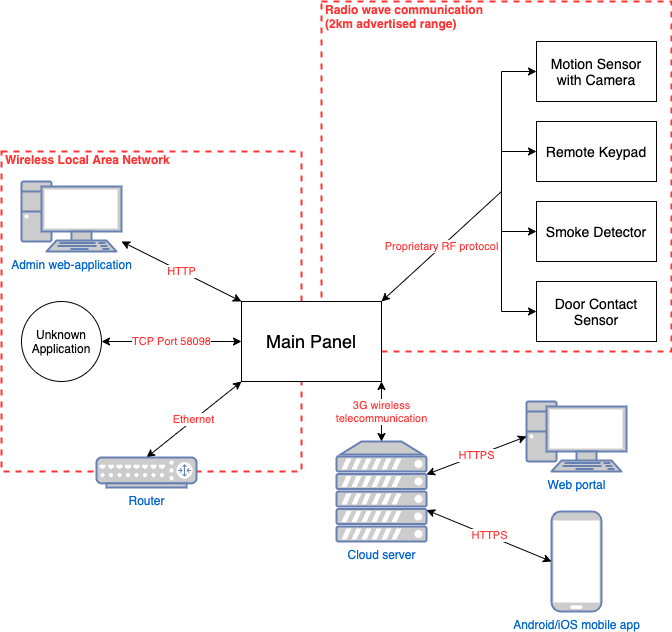
\includegraphics[width=\textwidth]{images/5-threat-model/system-overview.png}
    \caption{A data flow diagram of the system.}
    \label{fig:system-overview}
\end{figure}


\subsection{System Technologies}
Table \ref{tb:system-technologies} contains all identified technologies present in the system. There are undoubtedly additional technologies used but these are the ones identified and relevant.
\begin{table}[!p]
    \centering
    \begin{tabularx}{\textwidth}{l X}
        \hline
        \textbf{Technology}  & \textbf{Description}
        \\ \hline
        Main Panel & Linux 2.6-2.30. Hosts a web server over HTTP, using Mongoose (an embedded webserver), version unknown. Unknown application listening on TCP port 58098. Hosts DNS on TCP/UDP port 53. Has a USB and ethernet port.
        \\ \hline
        HTTP  & Protocol used by the admin web application. A clear text protocol used to communicate with the web admin panel.
        \\ \hline
        F1 RF protocol  & A proprietary \gls{RF} protocol from the hardware manufacturer, Climax Technology. Uses 868 MHz frequency. This is an undocumented protocol, meaning no technical specifications have been publicized.
        \\ \hline
        Mongoose web server  & An open-source web server, in C. Used by the main panel to host the local admin web page, version unknown. Information leaked via the HTTP \texttt{Server} header on some endpoints.
        \\ \hline
        ARM architecture  & The CPU of the main panel is an ARM (little-endian) SOC system from \textit{Grain Media}.
        \\ \hline
        3G telecommunication  & The main panel communicates with the external servers over the 3G mobile communication network.
        \\ \hline
        TCP  & The \gls{TCP} network protocol is used in communication. The main panel listens on three different TCP ports (53, 80, 58098).
        \\ \hline
    \end{tabularx}
    \caption{Technologies used in the system.}
    \label{tb:system-technologies}
\end{table}

\section{Decomposition of the system}
This section presents the results of the fourth step of the threat modeling technique. This includes all identified entry points of the system. Considering the architecture of the system, and the delimitations of this thesis, only the entry points of the main panel are presented.

As part of the decomposition of the system, all entry points of the system were identified. These are essentially all points of contact an attacker could probe. The entry points are documented in table \ref{tb:entry-points}.
\begin{table}[!ht]
    \centering
    \begin{tabularx}{\textwidth}{l X}
        \hline
        \textbf{Entry point} & \textbf{Description}
        \\ \hline
        Local web admin page  & See section \ref{ch:system:local-admin}. Provides very basic functionality but no control over the system. Has an undocumented login page via \textit{HTTP Basic Auth}. Data is transferred over HTTP on the local network.
        \\ \hline
        Unknown application  & This is a completely undocumented process, listening on TCP port 58098. Does not send any response.
        \\ \hline
        Main panel  & The physical device features an Ethernet port to connect to the local network, as well as a USB port for unknown purposes. It communicates with other devices over an 868 MHz proprietary \gls{RF} protocol.
        \\ \hline
        3G telecommunication  & The device has a SIM card and communicates over the 3G telecommunication network.
        \\ \hline
        \gls{RF} communication  & The device talks to the other peripherals over a proprietary \gls{RF} protocol, called \textit{F1}. There seems to be little to no information available to the public about this protocol, other than its operating frequency of 868 MHz.
        \\ \hline
        USB port  & The device has a USB 2.0 Type-A connector.
        \\ \hline
        Firmware  & The firmware of the system.
        \\ \hline
    \end{tabularx}
    \caption{The entry points of the main panel.}
    \label{tb:entry-points}
\end{table}

\section{Identified Threats} \label{ch:threat-model:threats}
\newcommand{\owaspref}[1]{OWASP IoT \##1}
\newcommand{\etsiref}[1]{ETSI \##1}

The following section contains all identified threats. These are categorized after the threat categories of the STRIDE model. For an explanation of the model and a description of each category see section \ref{ch:method:stride}. Note the additional category \textit{Supply chain issues}, which is a proposed extension to the model when threat modeling IoT devices \cite{guzman2017iot} (see section \ref{ch:method:threat-modeling}). The \textit{OWASP IoT top 10} \cite{owasp-iot-top10} was referenced to identify common threats that the system might be vulnerable to (see section \ref{ch:related-work:owasp}). In these threats, the OWASP IoT number is referenced as \textit{\owaspref{n}}. Similarly, the \textit{ETSI EN 303 645} standard \cite{etsi-iot-standard} for IoT manufacturers was used to identify threats (see section \ref{ch:related-work:etsi}). These are referenced below as \textit{\etsiref{n}}. Many of the threats related to the RF communication were identified through the references in section \ref{ch:related-work:hacking-iot} and \ref{ch:related-work:rf-exploit}.

\subsection{Spoofing Identity}
\begin{itemize}
    \item Spoof the remote keypad through the RF communication.
    \\ (\owaspref{7})
    \item Spoof the door contact sensor through the RF communication.
    \\ (\owaspref{7})
    \item Spoof the smoke detector through the RF communication.
    \\ (\owaspref{7})
    \item Spoof the motion detection camera through the RF communication.
    \\ (\owaspref{7})
    \item Spoof the remote keypad through the RF communication.
    \\ (\owaspref{7})
\end{itemize}

\subsection{Tampering with Data}
\begin{itemize}
    \item Replay attack on the RF communication through message blocking via jamming.
    \item Change and tamper with RF packets in transit.
    \item Send valid RF packets to the main panel, triggering events, without proper authorization.
    \\ (\owaspref{7}, \etsiref{5})
    \item Make the main panel fall back to its Ethernet connection instead of 3G telecommunication.
    \\ (\etsiref{9})
\end{itemize}

\subsection{Repudiation}
\begin{itemize}
    \item Replay attack on messages in the RF protocol between devices.
    \item Disrupt/disable logging of events.
\end{itemize}

\subsection{Information Disclosure}
\begin{itemize}
    \item Information leak in the packets of the \gls{RF} protocol.
    \\ (\etsiref{5})
    \item Weak or non-existent encryption in the \gls{RF} protocol.
    \\ (\etsiref{5})
    \item Password sniffing on the local webserver.
    \\ (\etsiref{5})
    \item Leaking the existence of the system by continuous RF traffic.
    \item Extracting firmware from the main panel.
    \\ (\owaspref{10})
\end{itemize}

\subsection{Denial of Service}
\begin{itemize}
    \item Jamming of the RF protocol.
    \\ (\etsiref{5})
    \item Stop the alarm from triggering until after you've left the premises.
    \item Spamming traffic to the local webserver.
    \\ (\owaspref{2})
    \item Crash the main panel or parts of the main panel.
    \\ (\etsiref{13})
    \item Crash the external devices through the RF communication.
    \\ (\owaspref{3}, \etsiref{13})
\end{itemize}

\subsection{Elevation of Privilege}
\begin{itemize}
    \item Insecure credentials used in the system.
    \\ (\owaspref{1}, \owaspref{9}, \etsiref{1})
    \item Password attack on the local webserver login page.
    \\ (\owaspref{1}, \owaspref{9})
    \item Send valid RF packets to the main panel without proper authorization.
    \\ (\owaspref{7})
    \item Gain an authenticated connection to the main panel through one of the network services.
    \\ (\owaspref{2}, \etsiref{6})
\end{itemize}

\subsection{Supply chain issues}
\begin{itemize}
    \item Using official applications from Climax Technology to access the system, like their mobile app Vesta Home 5 \footnotelink{https://play.google.com/store/apps/details?id=com.climax.vestasmarthome.eu}{2021-04-14}.
    \\ (\owaspref{3})
    \item Using debug applications from Climax Technology to access the system. These can be found on their website \footnotelink{https://climax.com.tw/downloads/}{2021-04-14}.
    \\ (\owaspref{3})
\end{itemize}
